\documentclass[12pt, twoside]{article}
% \documentclass[12pt, twoside]{article}
\usepackage[letterpaper, margin=1in, headsep=0.2in]{geometry}
\setlength{\headheight}{0.6in}
%\usepackage[english]{babel}
\usepackage[utf8]{inputenc}
\usepackage{microtype}
\usepackage{amsmath}
\usepackage{amssymb}
%\usepackage{amsfonts}
\usepackage[nomessages]{fp} %\FPeval{\var-name}{2*sin(pi/6)}
\usepackage{siunitx} %units in math. eg 20\milli\meter
\usepackage{yhmath} % for arcs, overparenth command
\usepackage{tikz} %graphics
\usetikzlibrary{quotes, angles, arrows, arrows.meta}
\usepackage{graphicx} %consider setting \graphicspath{{images/}}
\usepackage{parskip} %no paragraph indent
\usepackage{enumitem}
\usepackage{multicol}
\usepackage{venndiagram}

\usepackage{fancyhdr}
\pagestyle{fancy}
\fancyhf{}
\renewcommand{\headrulewidth}{0pt} % disable the underline of the header
\raggedbottom
\hfuzz=2mm %suppresses overfull box warnings

\usepackage{hyperref}
\usepackage{float}

\title{IB}
\author{Chris Huson}
\date{October 2025}

\fancyhead[LE]{\thepage}
\fancyhead[RO]{\thepage \\ First \& last name: \hspace{2.25cm} \,\\ Grade: \hspace{2.25cm} \,}
%\fancyhead[RO]{First \& last name: \hspace{2.25cm} \,\\ \,}
\fancyhead[LO]{La Scuola d'Italia / Huson / IB Math: Sequences \\* 31 October 2025}

\begin{document}

\subsubsection*{2.3 Classwork: Review; due Monday 3 November}
\begin{enumerate}[itemsep=0.25cm]

    \item Dr. Huson buys a new plant and measures how tall it is after a number of weeks. Some of his measurements are shown below. Plot the points in the grid below.
  \renewcommand{\arraystretch}{1.6}
    \begin{center}
      \begin{tabular}{|l|r|r|r|r|}
      \hline
      Weeks & 2 & 5 & 7 & 10\\
      \hline
      Height (cm) & 5 & 6 & 8 & 9 \\
      \hline
      \end{tabular}
    \end{center}

\begin{center} %4 quadrant regents grid w T-Chart
\begin{tikzpicture}[scale=.635]
  \draw [help lines] (0,0) grid (10,12);
  \draw [thick, ->] (0,0) -- (10.4,0) node [below right] {$Weeks$};
  \draw [thick, ->] (0,0)--(0,12.4) node [left] {$Height$};
  \node at (12,9)[right]{Check your calculator};
  \node at (12,8)[right]{$ax+b$};
  \node at (12,7)[right]{$a=0.529$};
  \node at (12,6)[right]{$b=3.82$};
  \node at (12,5)[right]{$r=0.976$};
\end{tikzpicture}
\end{center}
\begin{enumerate}[itemsep=1cm]
    \item State, rounding the coefficients to \emph{three significant figures}, the linear regression equation that approximates the height, $y$, of the plants after $x$ weeks.
    \item Explain what the $y$-intercept means in the context of the problem.
    \item Explain what the slope means in the context of the problem.
    \item Find the correlation coefficient, $r$. ``Characterize" the correlation between the two variables.
    \item Using the regression model, predict the height of the plant after 6 weeks.
\end{enumerate}

\newpage
\item Given that for a geometric sequence $u_1=54$ and $u_4=16$
\begin{enumerate}
    \item Find the value of $r$.
    \item Given that $u_k$ is the first term of the sequence with a value less than one, find $k$.
    \item Find the sum of the infinite series $S_\infty$
\end{enumerate}

\item The first three terms of an arithmetic sequence are $u_1=7.1$, $u_2=7.4$, and $u_3=7.7$.
\begin{enumerate}
    \item Find the common difference.
    \item Given that the $k$th term of the sequence, $u_k=11$. Find $k$.
\end{enumerate}

\item Let $x=\ln 3$ and $y=\ln 7$. Write down the following expressions in terms of $x$ and $y$.
\begin{enumerate}
    \item $\ln \frac{7}{3}$
    \item $\ln 63$
    \item $\ln 9$
\end{enumerate}

\item Let $f(x) = x^2-8x+3$
\begin{enumerate}
    \item Rewrite quadratic in vertex form and state the vertex as an ordered pair.
    \item The parabola is translated vertically by $k$ units to make the function $g(x)$. The equation $g(x)=0$ has one solution. Find $k$.
\end{enumerate}

\item The function $g$ is defined by graph of $y=g(x)$ below.
\begin{enumerate}
    \item Write down the equation for $g(x)$ in factored form.
    \item The function $h(x)$ is made by reflecting $g$ across the $x$-axis. What is the equation for $h(x)$?
\end{enumerate}

\begin{figure}[!ht]
    \centering
    \includegraphics[width=0.4\textwidth]{../graphics/parabola-graphic.pdf}
\end{figure}
       
\end{enumerate}
\end{document}
